\documentclass[10pt,twocolumn,letterpaper]{article}

\usepackage{statcourse}
\usepackage{times}
\usepackage{epsfig}
\usepackage{graphicx}
\usepackage{amsmath}
\usepackage{amssymb}

% Include other packages here, before hyperref.

% If you comment hyperref and then uncomment it, you should delete
% egpaper.aux before re-running latex.  (Or just hit 'q' on the first latex
% run, let it finish, and you should be clear).
\usepackage[breaklinks=true,bookmarks=false]{hyperref}


\statcoursefinalcopy


\setcounter{page}{1}
\begin{document}


%%%%%%%%%%%%%%%%%%%%%%%%%%%%%%%%%%%%%%%%%%%%%%%%%%%%%%%%%%%%%%%
% DO NOT EDIT ANYTHING ABOVE THIS LINE
% EXCEPT IF YOU LIKE TO USE ADDITIONAL PACKAGES
%%%%%%%%%%%%%%%%%%%%%%%%%%%%%%%%%%%%%%%%%%%%%%%%%%%%%%%%%%%%%%%



%%%%%%%%% TITLE
\title{SBE304 Team 9 Echocardiogram Project Proposal}

\author{Ahmed Mahdy Mohammed Ali\\
{\tt\small Ahmedmahdy3098@gmail.com}
\and
Adel Refat Ali Elnahas\\
{\tt\small adel.elnahas97@eng-st.cu.edu.eg}
\and
Yossef Sameh Mohammed\\
{\tt\small yossefsameh23@gmail.com}
\and
Mahmoud Abd El-monem\\
{\tt\small thirdauthor@eng-st.cu.edu.eg}
}

\maketitle
%\thispagestyle{empty}



% MAIN ARTICLE GOES BELOW
%%%%%%%%%%%%%%%%%%%%%%%%%%%%%%%%%%%%%%%%%%%%%%%%%%%%%%%%%%%%%%%



%%%%%%%%% BODY TEXT



%\begin{itemize}
%	\item The information in this template is very minimal, and this file should serve you as a framework for writing your proposal. You may prefer to use a more collaboration-friendly tool while drafting the report with your class mates before you prepare the final report for submission. Remember that you should \textbf{submit both the report and code} you used for this project via Canvas. Also, \textbf{only one member per team} needs to submit the project material.
%	
%	\item The project proposal is a 2-4 page document excluding references\footnote{This means, references should of course be included but do not count towards the page limit}.
%	
%	\item You are encouraged (not required) to use 1-2 figures to illustrate technical concepts.
%	
%	\item The proposal must be formatted and submitted as a PDF document on Canvas (the submission deadline will be later announced via the schedule \& email).
%	
%	\item Please
%	check out the text in these sections for further information.
%	
%\end{itemize}

%


\section{Introduction}

Many patients have suffered heart attacks at some point in the past. Some are still alive and some are not. The survival and still-alive variables, when taken together, indicate whether a patient survived for at least one year following the heart attack.

What we are planning to do is given the dataset at hand,We'll use some machine learning classifiers to predict whether or not the patient will survive at least one year. 

Using various porbability methods to ensure the most accurate results.

The problem addressed by past researchers was to predict from the other variables whether or not the patient will survive at least one year. The most difficult part of this problem is correctly predicting that the patient will NOT survive. (Part of the difficulty seems to be the size of the data set.)

%In this section, describe what you are planning to do. Also, briefly describe related work.


%When discussing related work, do not forget to include appropriate references.  This is an example of a %citation \cite{mirjalili2018gender}. To format the citations properly, put the
%corresponding references into the bibliography.bib file. You can obtain
%BibTeX-formatted references for the "bib" file from Google Scholar 
%(\url{https://scholar.google.com}), for example, by clicking on the 
%double-quote character under a citation and then selecting \mbox{"BibTeX"} as
%shown in Figure \ref{fig:google-scholar-1col} and 
%Figure \ref{fig:google-scholar-2col}.


%\begin{figure}[t]
%\begin{center}
 %  \includegraphics[width=0.8\linewidth]{figures/google-scholar.pdf}
%\end{center}
  % \caption{Example illustrating how to get BibTeX references from
 %  Google Scholar as a 1-column figure.}
%\label{fig:google-scholar-1col}
%\end{figure}


%\begin{figure*}
%\begin{center}
 %  \includegraphics[width=0.8\linewidth]{figures/config-texmaker.png}
%\end{center}
 %  \caption{Compiling this document using \emph{TexMaker}.}
%\label{fig:google-scholar-2col}
%\end{figure*}


\section{Motivation}

What is interesting about this project is what can be achieved using probability and statistical models
in healthcare.


\section{Evaluation}
		
		
It can be used to evaluate the probability of survival of a patient and given the results, proceed with the appropriate actions.

A successful project would have a logical and realistic outcome.

Measuring success should be based on data manuplation (normalization and imputation) and proper using of classification methods.
		\linebreak
		  Methods:
		
\begin{itemize}
		
		\item Naive Bayes (NB) Classier (or Gaussian NB Classifier)
		\item Decision Trees
		\item Logistic regression
\end{itemize}




\section{Exploratory data analysis (EDA)}
As shown in the Figure
We will be using data visualization (histogram) using R programming (ggplot) to display different data.


	\begin{figure}[t]
		\begin{center}
   			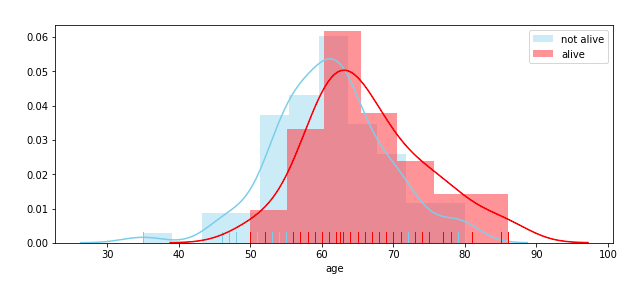
\includegraphics[width=0.8\linewidth]{figures/histogram.png}
		\end{center}
   		\caption{Example of data visualizations}
   
		\label{fig:histogram}
	\end{figure}

\section{Resources}
\begin{itemize}
 \item Dataset \cite{kaggle} \footnote{\url{https://www.kaggle.com/loganalive/echocardiogram-uci/metadata}}.
	
	
\end{itemize}
%What resources are you going to use (datasets, computer hardware, computational tools, etc.)?

\section{Contributions}

You are expected to share the workload evenly, and every group member is expected to participate in both the experiments and writing. (As a group, you only need to submit one proposal and one report, though. So you need to work together and coordinate your efforts.)

Clearly indicate what computational and writing task each member of your group will be participating in.




\pagebreak

\section{Publicity}




	Authors' Personal websites



\begin{itemize}
	\item Adel Refat \footnote{\url{https://adel-elmala.github.io}}
	\item Ahmed Mahdy \footnote{\url{https://amahdy98.github.io}}
	\item Youssef samed \footnote{\url{https://yossefsameh.github.io/YossefSameh}}
	\item Mahmoud Abd Elmonem \footnote{To be added}
\end{itemize}
{\small

\bibliographystyle{IEEEtran}
\bibliography{bibliography.bib}
}
\end{document}
